\section{Level-1 Trigger}
\label{sec:l1trigger}

In order to cope with the high collision rate, a two-tier trigger
system is implemented at CMS. The trigger is able to use 
limited information from each event to decide whether or not
to record the event. This allows a large reduction in the rate
of data-taking while maintaining a high efficiency to select events
producing interesting physics objects.
The first level, the Level-1 (L1) trigger, uses custom-built 
electronics in order to reduce the output rate from 40 MHz to 100 kHz~\citep{l1}.
Events which satisfy some relatively loose set of criteria are passed to 
the second level, the high-level trigger (HLT), where more sophisticated
algorithms, much closer to those used in the offline reconstruction,
are used to decide whether or not to store an event~\citep{hlt}.

The L1 calorimeter trigger is able to
use coarse measurements of the energy deposited in the ECAL and HCAL
to form candidate physics objects such as electrons, photons, tau leptons
decaying hadronically and hadronic jets. With the exception of 
electrons and photons, all of the L1 algorithms run in the Global Calorimeter
Trigger (GCT).  The following section is a description of 
a set of calibrations for the GCT designed to improve the resolution of 
the L1 jets.  

\subsection{Jet Energy Calibration}
\label{sec:jetenergyresponse}
The response of the hadronic calorimeter varies
considerably across its barrel, endcap and forward sections. 
The energies of jets are corrected offline to account for these effects;
however, if left uncalibrated at L1, this can lead to inefficiencies in the 
trigger system. The response is measured in QCD Monte Carlo (MC)
simulation by comparing the $p_{T}$ of L1 jet candidates to generated
jets. The generated jets are reconstructed using an anti-$k_{T}$ jet finding algorithm~\citep{antikt}. 
L1 jets are matched
to generator jets by determining the minimum separation, $\Delta R$, between 
each generator jet and any L1 jet candidate and requiring it be less than 0.7.
This is much looser than typical matching requirements applied offline due to the coarser
spatial resolution of the L1 jets.
The generator and the closest of these L1 jets is defined as a matched pair
and the response is calculated as $\Lonept/\Genpt$ for that pair.
Figure~\ref{fig:respvseta} shows the response as a function of the pseudo-rapidity of the
generated jet $|\Geneta|$.

\begin{figure}
\begin{center}
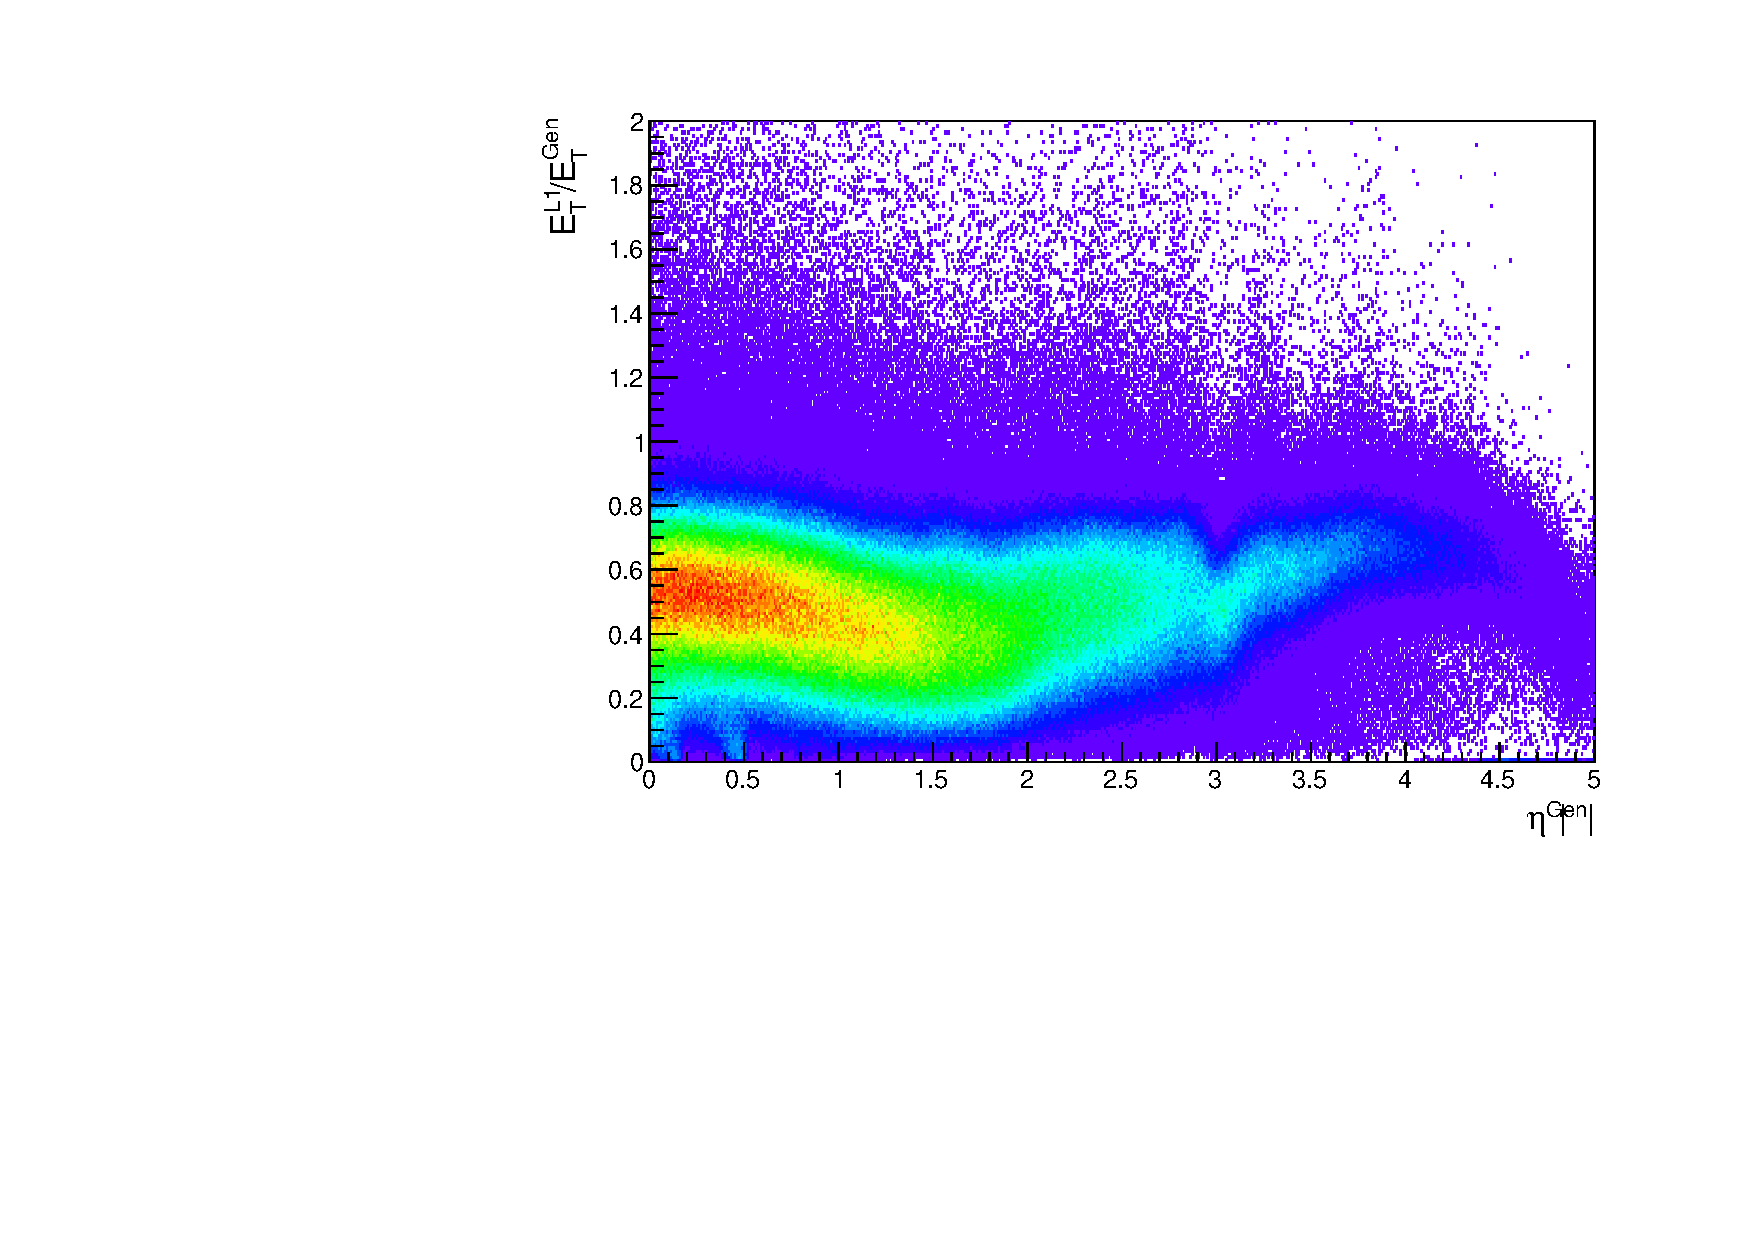
\includegraphics[width=.8\textwidth]{detector/l1jet/bias.pdf}
\caption{Response measured from matched generator-L1 jet pairs in MC 
	as a function of the generator jet pseudo-rapidity $|\Geneta|$.}
\label{fig:respvseta}
\end{center}
\end{figure}

The response is measured in 11 $|\eta|$ bins which correspond to the 11 GCT regions.
Corrections for each region are derived as a function of $\Lonept$ by determining 
the average response, $\left<\Lonept/\Genpt\right>$, and $\left<\Lonept\right>$
in 4 GeV bins of $\Genpt$ between 14 GeV and 200 GeV. Below 14 GeV, the resolution in $\Lonept$ restricts
a proper measurement of the response while above 200 GeV, the response approaches unity.
The average response is taken from the mean of a 
Gaussian fit to the distribution of $\Lonept/\Genpt$ while $<\Lonept>$ is taken as the mean 
average of the $\Lonept$ distribution. For low values of $\Genpt$, the response becomes very non-Gaussian
due to the limited resolution of the L1 trigger, so in this case, the average response is taken
as the mean of the $\Lonept/\Genpt$ distribution. The response is inverted to provide a
corrective scale factor in each region as a function of $\Lonept$. This is then parameterised 
by performing a chi-squared fit of the functional form given in Equation~\ref{eqn:jecfit}.

\begin{equation}
\left<\Lonept/\Genpt\right>^{-1} = \Lonept \cdot \left ( p_{0} + 
\frac{p_{1}}{(\log \Lonept)^{2}+p_{2}}+p_{3} \exp(-p_{4}
(\log \Lonept-p_{5} ) ^{2}) \right )
\label{eqn:jecfit}
\end{equation}

The functional form chosen provides a good description of the shape at low $\Lonept$ in the high $|\eta|$ regions 
and is the same as that used for offline jet calibration at CMS~\citep{jetcalib}.
The parameterisation provides a multiplicative correction to be applied to L1 jets online. 
Figure~\ref{fig:egcorrfunc} is an example of the fit in the $0.348 < |\Geneta| < 0.695$ bin.
The full set of fits in each of the 11 $\Genpt$ bins can be found in Appendix~\ref{app:jecfits}.

\begin{figure}
\begin{center}
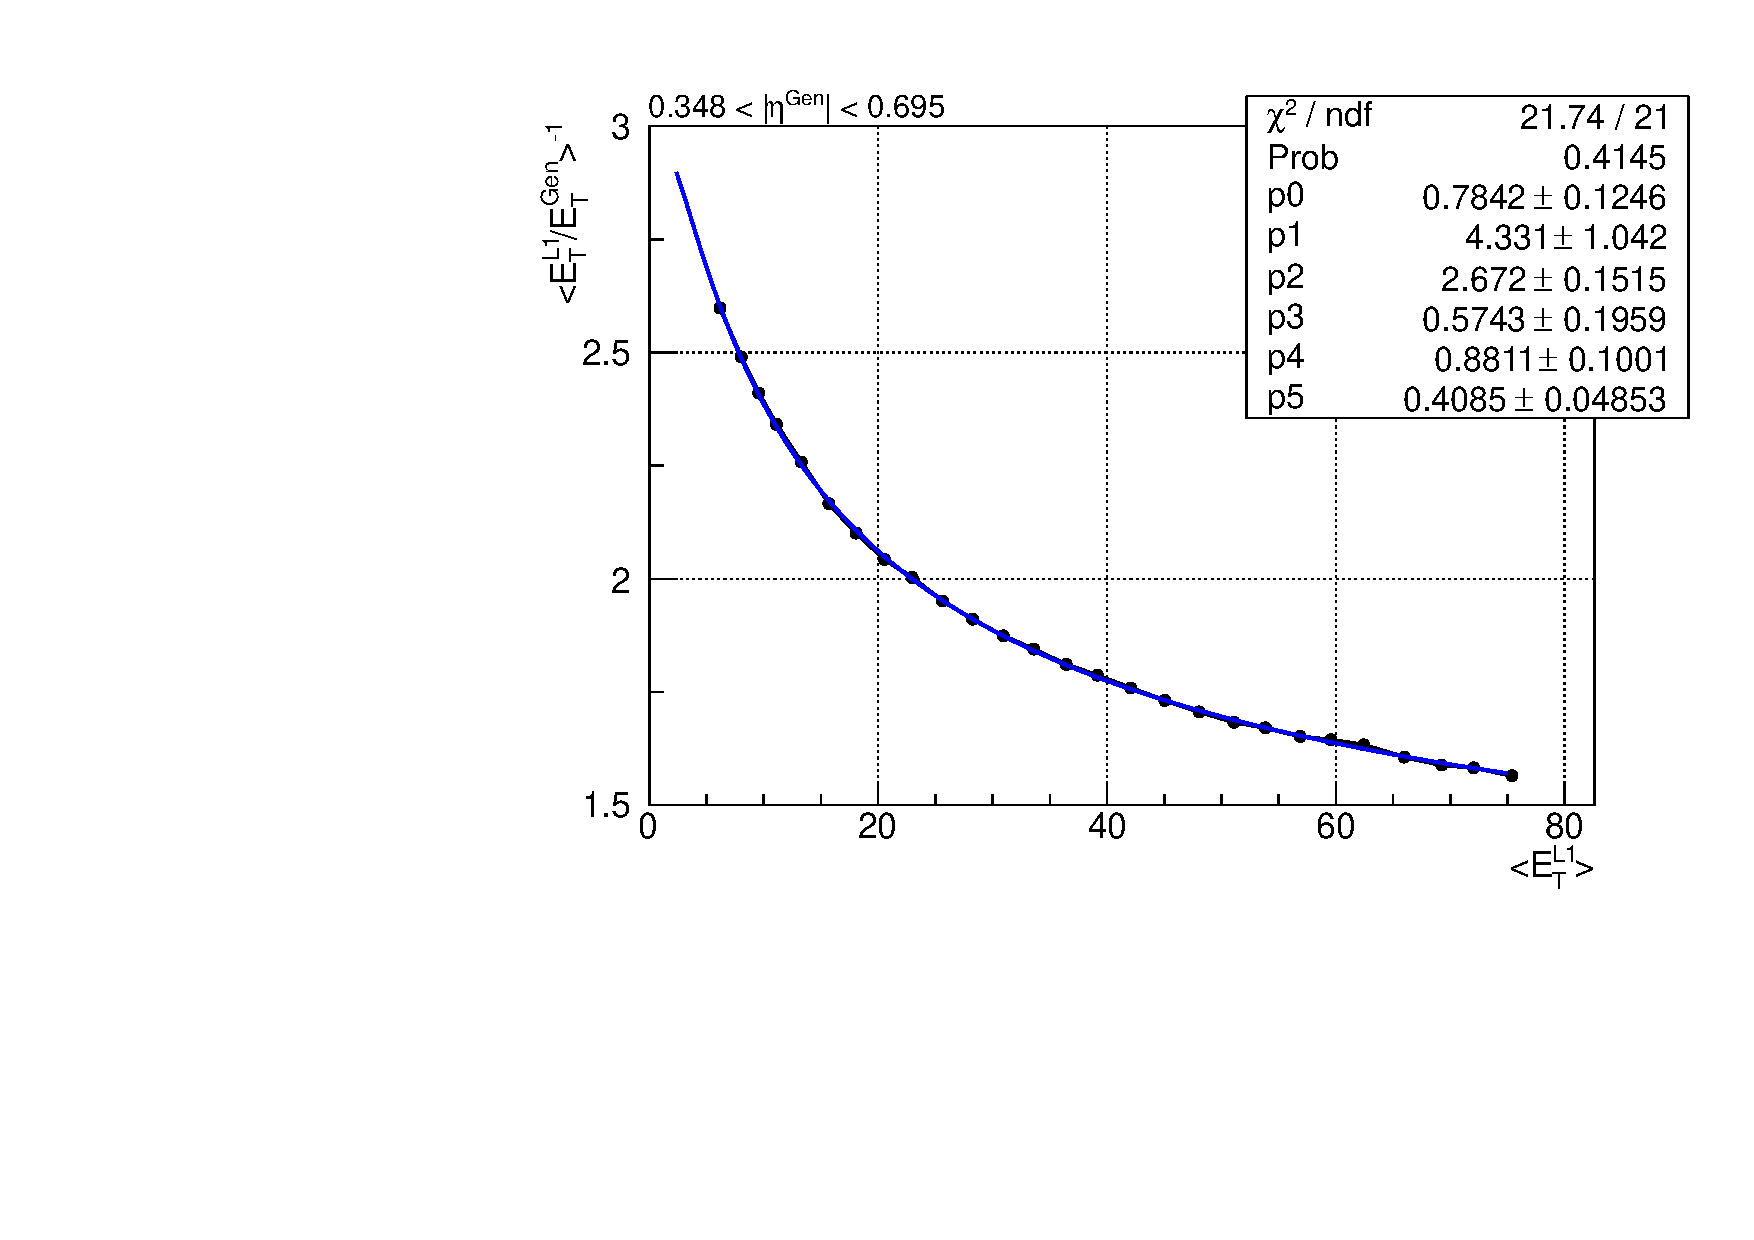
\includegraphics[width=0.8\textwidth]{detector/l1jet/egcorrfunc.pdf}
\end{center}
\caption{Correction function for the $0.348 < |\Geneta| < 0.695$. The points represent the average
quantities as measured in MC. The blue line is a parametric fit to the points 
using a chi-squared minimisation. The error bars, estimated from the number of MC events, are too small 
to be visible in this plot.}
\label{fig:egcorrfunc}
\end{figure}

\subsection{Calibration Performance}
The calibrations derived were applied using the GCT emulation software to the same MC sample 
used to derive them to provide a closure test of their performance. 
The response is shown in Figure~\ref{fig:closure}
as a function of $\Lonept$ and $\Geneta$. The points in each figure are calculated from a Gaussian fit to the distribution
of $\Lonept/\Genpt$ in bins of $\Lonept$ and $\Geneta$ respectively. 
The results show that the procedure closes
to a precision of between 5\% and 10\%. The improvement in L1 jet resolution expected from MC
is demonstrated in Figure~\ref{fig:mcresolutionl1}. The resolution, calculated by fitting a Gaussian to the distribution
of the difference in $E_{T}$ measured at L1 to that of the generator jet 
in bins of $\Lonept$ (see Appendix~\ref{app:closurefits}), for L1 jets is shown before and after applying the
corrections. 
 
\begin{figure}
\begin{center}
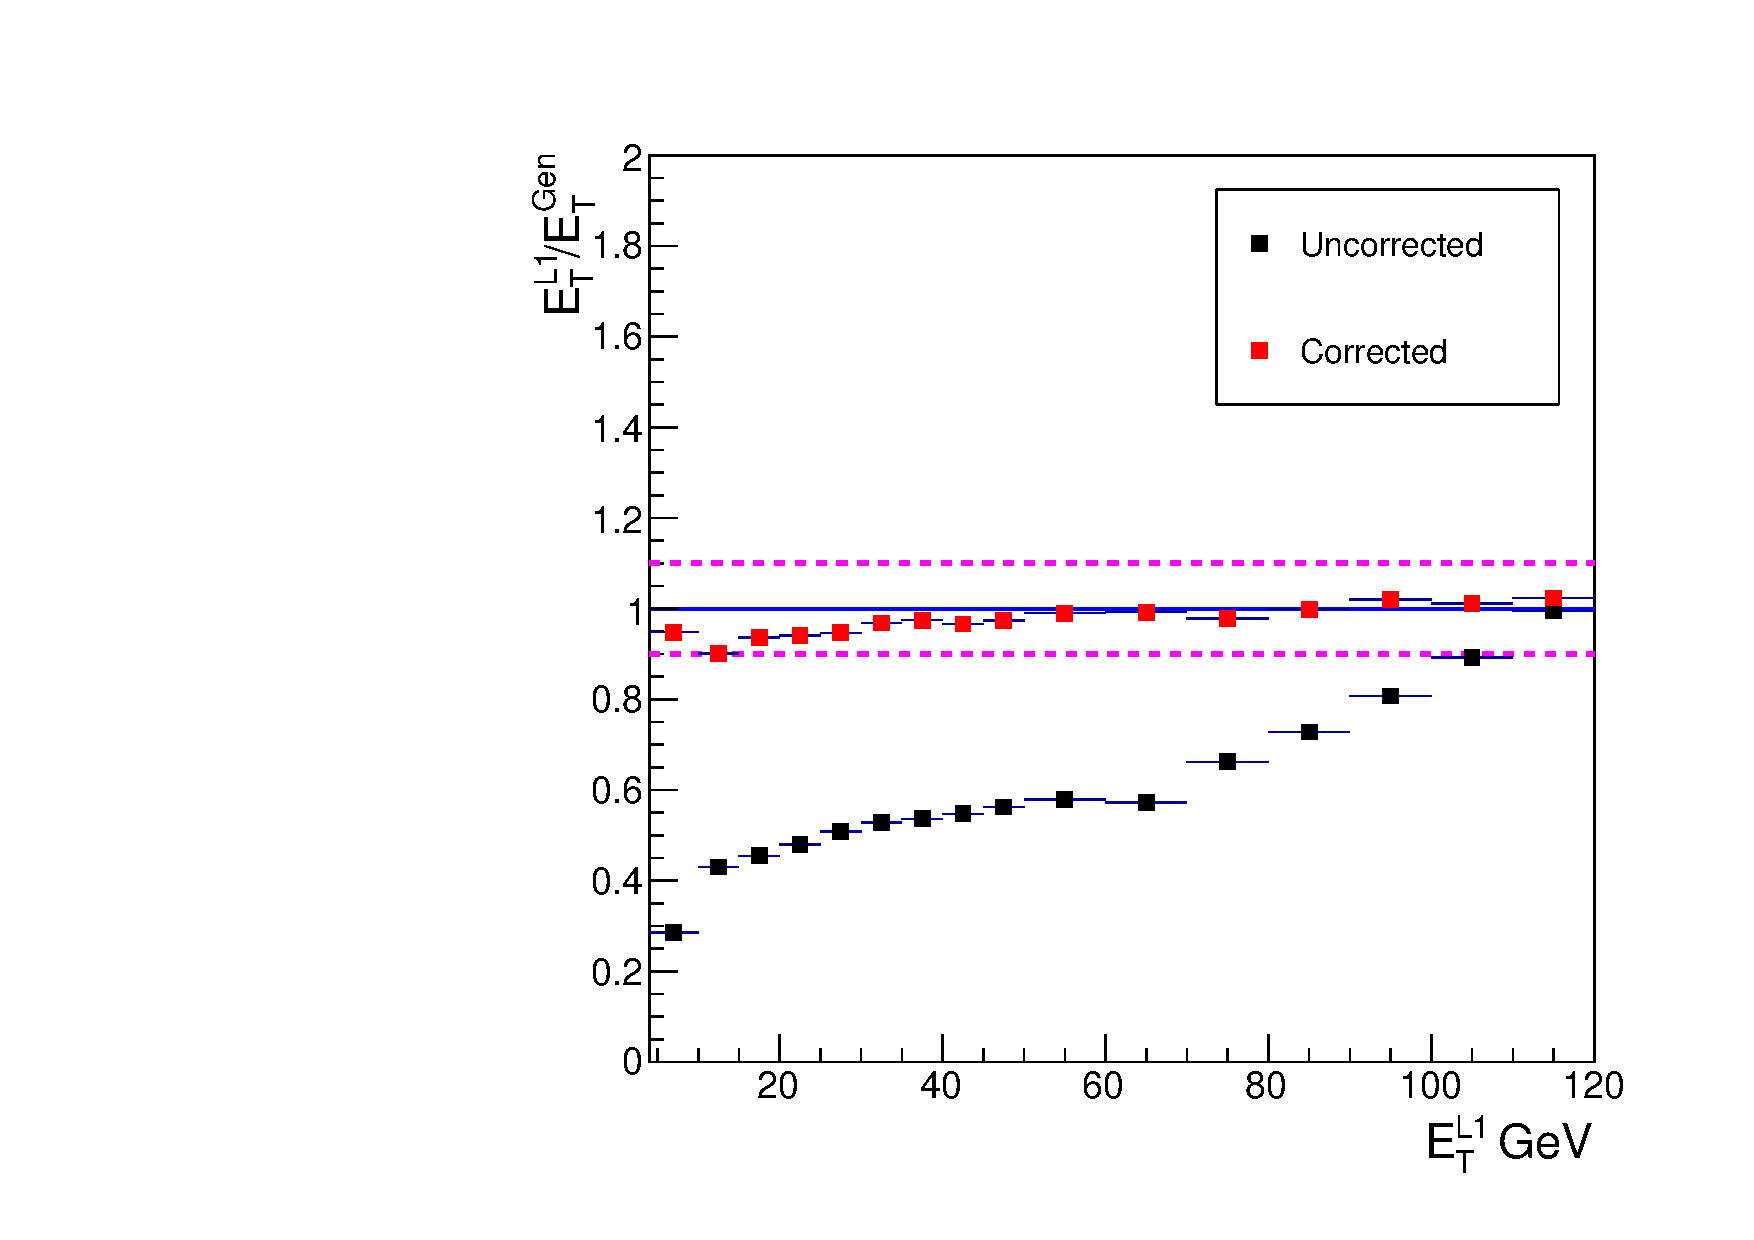
\includegraphics[width=0.49\textwidth]{detector/l1jet/rspvspt.pdf}
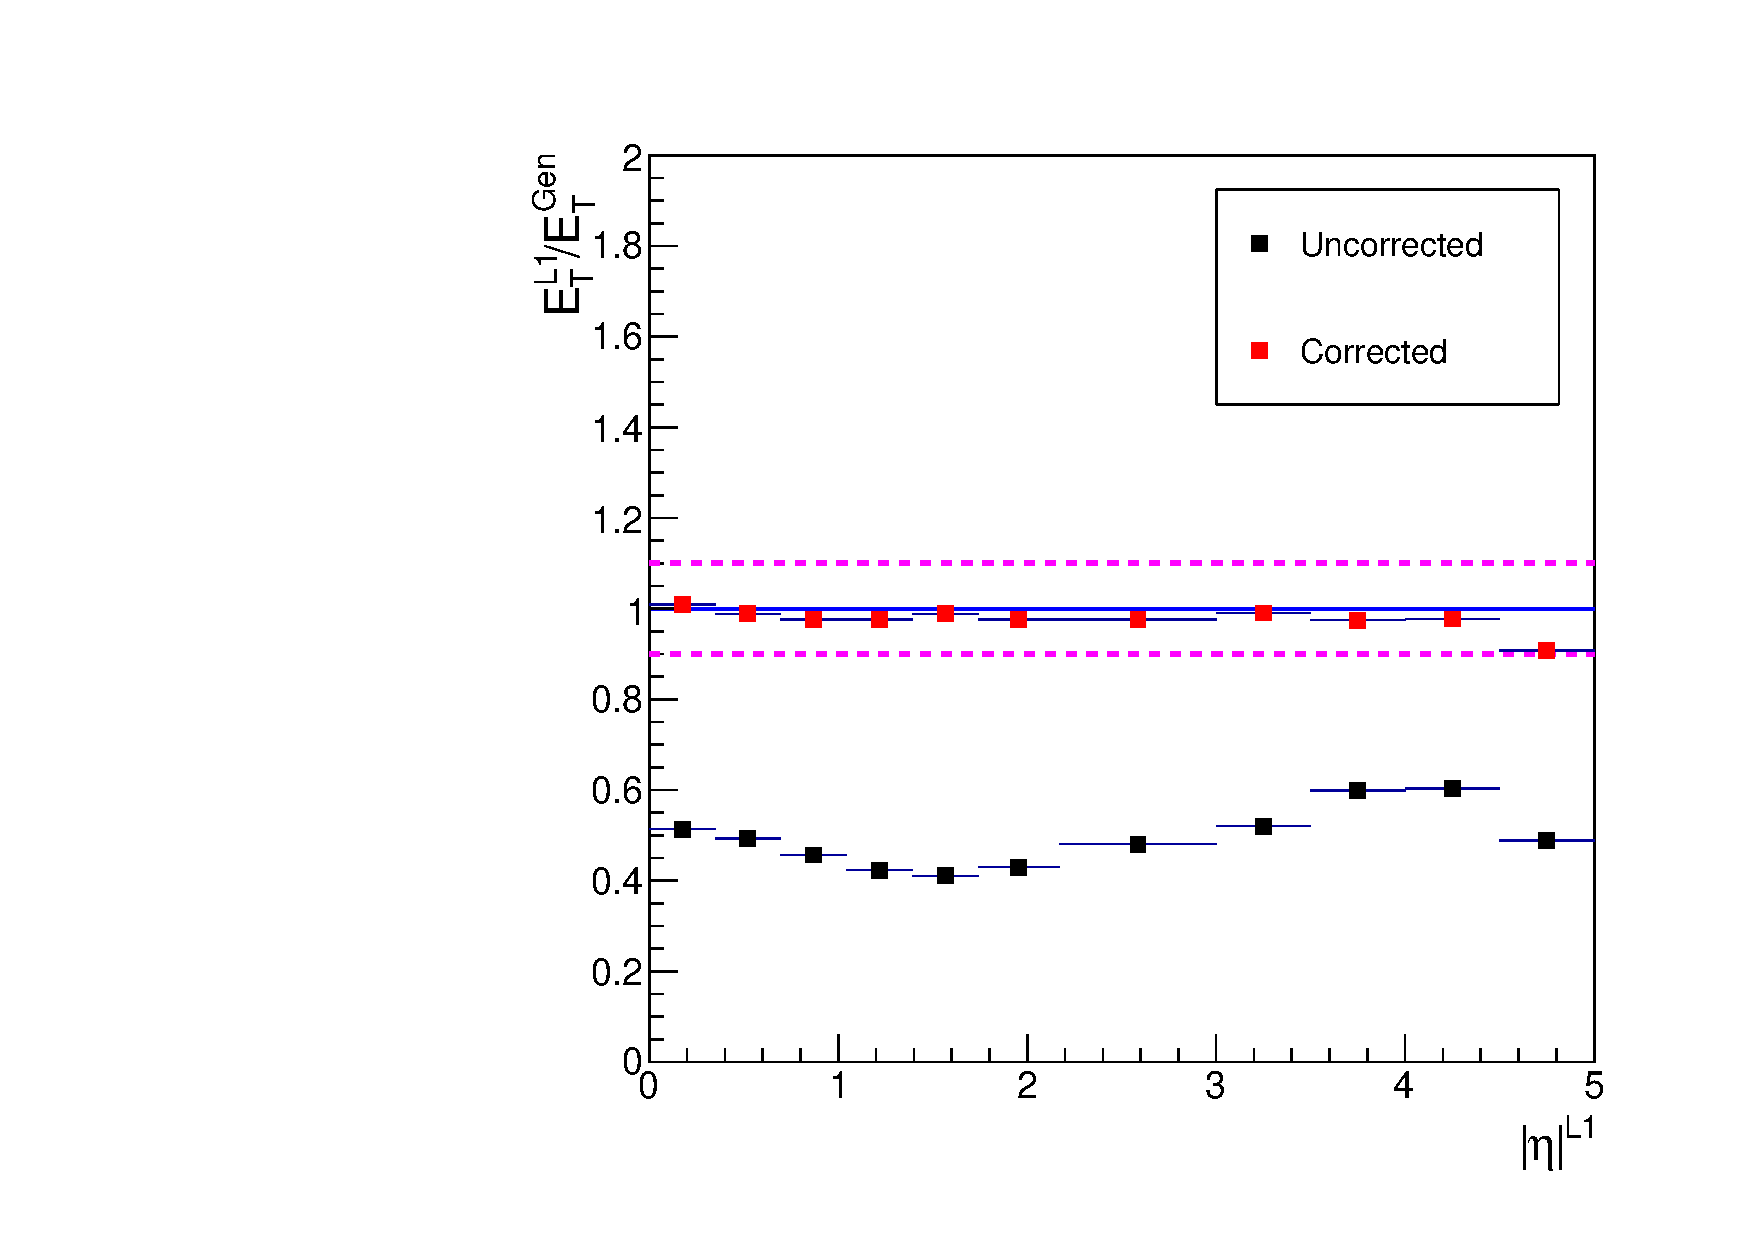
\includegraphics[width=0.49\textwidth]{detector/l1jet/rspvseta.pdf}
\end{center}
\caption{Closure tests performed in MC as a function of $\Lonept$ (left) and $\Geneta$ (right). 
The test shows that after applying the corrections, the response is within 10\% (dashed lines) of unity. 
The error bars are too small to be visible in these plots.}
\label{fig:closure}
\end{figure}

\begin{figure}
\begin{center}
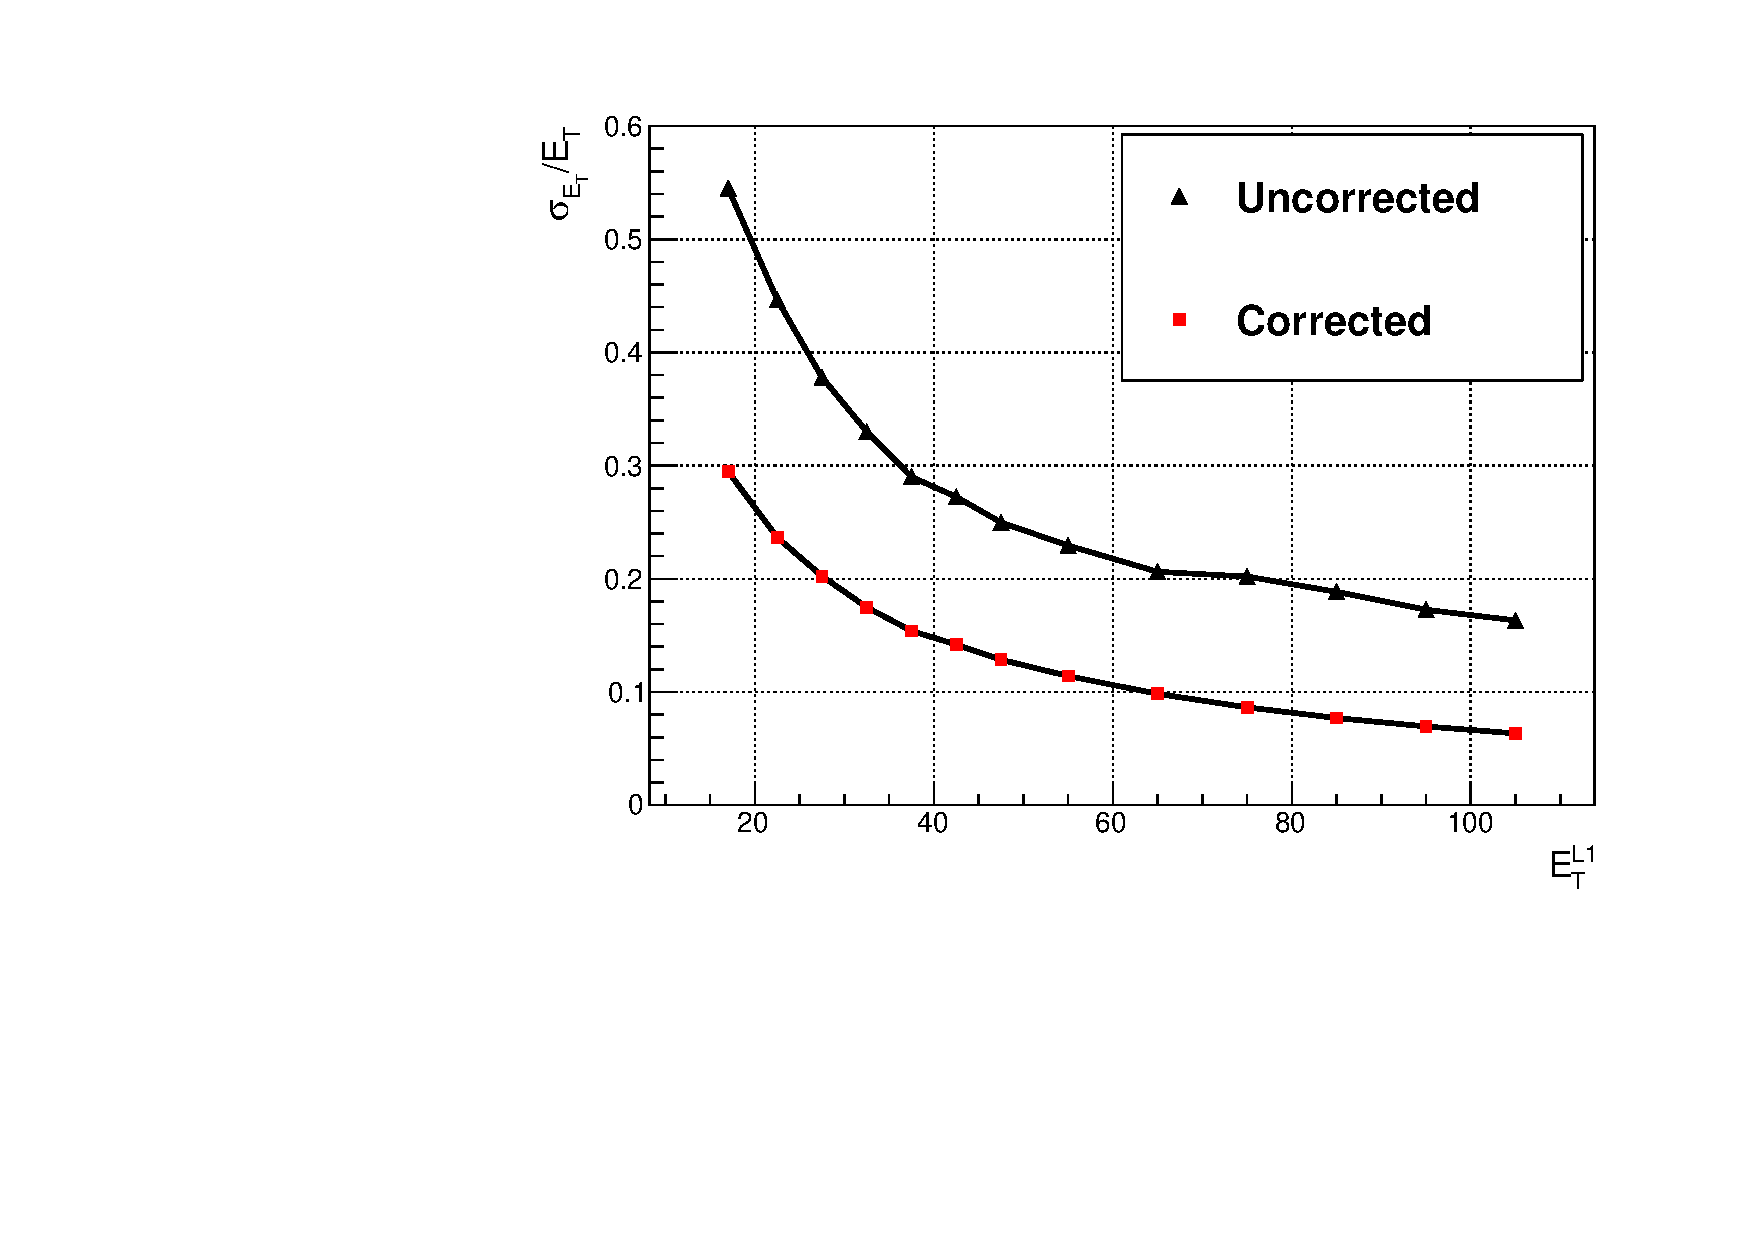
\includegraphics[width=0.8\textwidth]{detector/l1jet/MCresolution.pdf}
\end{center}
\caption{Jet energy resolution at L1 as a function of $\Lonept$ before and after application of the derived calibrations.
 The error bars are too small to be visible in these plots.}
\label{fig:mcresolutionl1}
\end{figure}


\subsubsection{Performance in Data}
The corrections derived in MC were applied to data online during and since run 2011B.
The resolution as a function of $\Lonept$ was measured using events in data from that run period
using the following method.
First, the fraction of L1 jets above some threshold in $\Lonept$ is determined as a function 
of the fully reconstructed jet $E_{T}$ in data.  
This is then fit with an error function of the form, 
\begin{equation}
\mathrm{erf}(x)\propto \int_{0}^{\frac{x-\mu}{\sigma}} e^{-t^{2}}dt,
\end{equation}
to provide a measure of the average energy in the calorimeters 
for jets which just pass the threshold at L1 ($\mu$) and the resolution of those jets ($\sigma$). 
As the full energy reconstruction for jets at CMS is much
more accurate than the value reconstructed at the L1 trigger, the effects of the jet energy resolution
after applying the full jet reconstruction are negligible. This is repeated for different thresholds in $\Lonept$.
Figure~\ref{fig:l1dataresolution} shows the resolution as a function
of $E_{T}$, where the value of $E_{T}$ is taken from the $\mu$ parameter of each fit. 
The uncertainties on each point represent the statistical uncertainty from the error function fits.
The points are fit with the parameterisation given in Equation~\ref{eqn:resofit} to extract the parameters which describe the
resolution of the calorimeter. The energy resolution of the L1 jets is improved after applying these 
calibrations in the GCT~\citep{l1triggernote}.
%An independent set of corrections were derived and applied during Run2011A but 
%were found to give worse performance than the ones described here in particular for jets with 
%$E_{T}>130$ GeV. 

\begin{figure}
\begin{center}
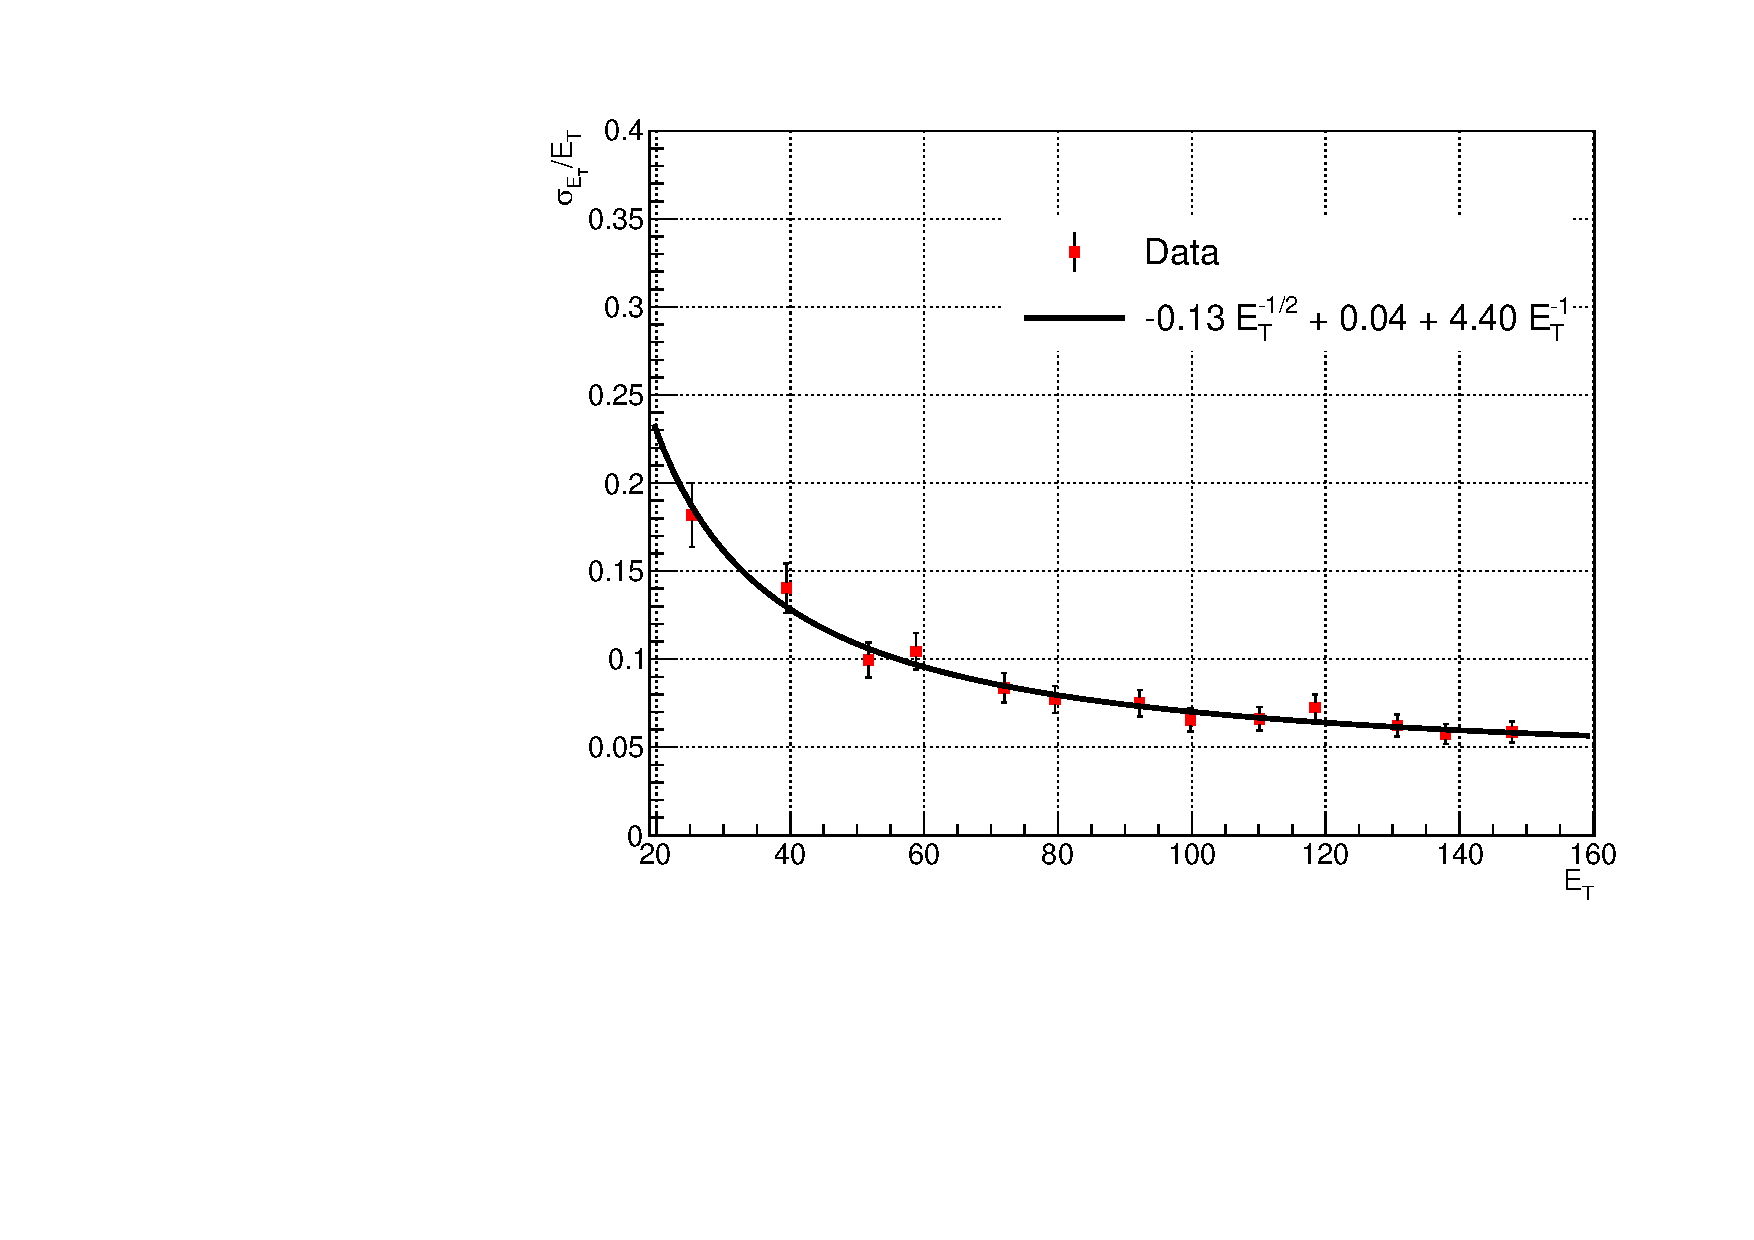
\includegraphics[width=0.8\textwidth]{detector/l1jet/DataResolution.pdf}
\end{center}
\caption{Energy resolution, $\sigma_{E}$, of L1 jets as a function of transverse energy deposited in the
calorimeter, $E_{T}$. The coefficients of the functional form shown are the result of a fit to the points.}
\label{fig:l1dataresolution}
\end{figure}



